\documentclass[
	parskip=half,
	a4paper,
]{scrarticle}

\usepackage{xcolor}
\definecolor{seeblau}{HTML}{00A9E0}
\definecolor{seegrau}{HTML}{9AA0A7}

\definecolor{seeblau1}{HTML}{CCEEF9}
\definecolor{seeblau2}{HTML}{A6E1F4}
\definecolor{seeblau3}{HTML}{59C7EB}
\definecolor{seeblau4}{HTML}{00A9E0}
\definecolor{seeblau5}{HTML}{008ECE}


\usepackage{graphicx}
\usepackage{amsmath}
\usepackage{subcaption}
\usepackage{wrapfig}
\usepackage[english]{babel}
\usepackage{blindtext}
\usepackage{microtype}
\usepackage{siunitx}
\usepackage[utf8]{inputenc}
\usepackage{csquotes}
\usepackage{nicefrac}
\usepackage[T1]{fontenc}
\usepackage{amsfonts}
\usepackage{amssymb}
\usepackage{tikz}
\usepackage{parskip}

\usepackage{libertinus, libertinust1math}
\usepackage[sfdefault]{biolinum}
\usepackage{roboto}

\setkomafont{disposition}{\normalfont\sffamily}

% set margins
\usepackage{geometry}
\geometry{
	a4paper,
	left=2.5cm,
	right=2.5cm,
	top=2.5cm,
	bottom=2.5cm
}

% caption
\usepackage{caption}
\captionsetup{
	% font={sf},
	labelfont={sf, bf, color=seeblau},
	labelsep=quad,
	labelformat=simple,
}

% links
\usepackage{hyperref}
\hypersetup{
	colorlinks=true,
	linkcolor=seeblau,
	citecolor=seeblau,
	urlcolor=seeblau,
	% hidelinks=true
}

% bibliography
\usepackage[
	style=numeric-comp, % comp = compressed 4,5,6,7 -> 4-7
	sorting=none,		% Sort by appearance
	% autocite = superscript,
	% backref=true,
	hyperref=true,
	url=true,
	maxbibnames=100
]{biblatex}

\usepackage{float}
% \floatplacement{figure}{h}
% \floatplacement{table}{H}

% loosen float placement rules
\renewcommand{\topfraction}{0.8}
\renewcommand{\bottomfraction}{.8}
\renewcommand{\textfraction}{0.1}
\renewcommand{\floatpagefraction}{.9}
% make floats less likely to be placed on a separate page
\setcounter{totalnumber}{9}
\setcounter{topnumber}{9}
\setcounter{bottomnumber}{9}

% decrease space between floats and text
\setlength{\textfloatsep}{0.25cm}
\setlength{\floatsep}{0.25cm}

% decrease space after disposition
\RedeclareSectionCommands[
	afterskip=1px
]{section, subsection, subsubsection}

\usepackage{adjustbox}

\usepackage{datetime}
\newdateformat{dotdate}{
	\twodigit{\THEDAY}.\twodigit{\THEMONTH}.\THEYEAR
}
\newdateformat{monthyeardate}{%
  \monthname[\THEMONTH] \THEYEAR}


% header and footer
\usepackage[
  markcase=noupper
]{scrlayer-scrpage}% activates pagestyle scrheadings automatically
\clearpairofpagestyles
\setkomafont{pageheadfoot}{\normalfont\sffamily}
\setkomafont{pagenumber}{\normalfont\sffamily}
% \chead*{\color{seegrau} Draft \dotdate\today}
\ofoot*{\pagemark}
\ohead*{\rightmark}


\usepackage{ifthen}
\newcommand{\markieren}[4]{
	\ifthenelse{\equal{#1}{}}{}{\adjustbox{padding=3pt, bgcolor=seeblau1, margin=-1pt}{\strut{\sffamily\robotoMedium{#1}}}\\}
  \ifthenelse{\equal{#2}{}}{}{\adjustbox{padding=3pt, bgcolor=seeblau2, margin=-1pt}{\strut{\sffamily\robotoMedium{#2}}}\\}
	\ifthenelse{\equal{#3}{}}{}{\adjustbox{padding=3pt, bgcolor=seeblau3, margin=-1pt}{\strut{\sffamily\robotoMedium{#3}}}\\}
	\ifthenelse{\equal{#4}{}}{}{\adjustbox{padding=3pt, bgcolor=seeblau4, margin=-1pt}{\strut{\sffamily\robotoMedium{#4}}}}
}

\addbibresource{../literature.bib}
\begin{document}

\title{Hot-Electron Emission for Spectral Calibration}
\author{Leon Oleschko}
\date{\dotdate\today}

\begin{titlepage}
    \sffamily
    \vspace*{3cm}
    {
        \fontsize{32}{32}
        \markieren{}{}{Hot-Electron Emission}{for Spectral Calibration}
    }
    \vspace{.25cm}\\
    {
        \Large
        Leon Oleschko\\
        Supervised by Peter Baum
        \vspace{.05cm}\\
        \dotdate\today\\
        % \vspace{.25cm}\\
        % \normalsize
        Universität Konstanz
    }
    \vfill
    {
        \normalfont\normalsize

    }
    \vfill
    \begin{flushright}
        Available at \url{www.github.com/leoole100/projekt-praktikum}.
    \end{flushright}
\end{titlepage}

% {
% 	\sffamily
% 	\hypersetup{hidelinks}
% 	\tableofcontents
% }

\clearpage

\section{Introduction}
Accurate spectral measurements require knowledge of an instrument’s spectral response—how efficiently the system transmits and detects light as a function of wavelength. To recover physically meaningful spectra, the system response must be determined against a known reference and applied as a correction.

This work targets the ultraviolet (UV), where suitable calibration sources are limited. Deuterium lamps are the practical standard in the UV because of their strong output below about \SI{350}{\nano\metre}, yet their spectral irradiance is markedly wavelength dependent and subject to aging and stability issues. Primary radiometric scales are realized using high-temperature graphite-cavity blackbodies operated near $\sim$\SI{3500}{\kelvin} and propagated via calibrated transfer standards to working instruments \cite{yoon_nist_2011,sapritsky_black-body_1995}.

In a lamp-based calibration, a source with known spectral irradiance is measured at the spectrometer input to solve for the instrument’s wavelength-dependent response. In the UV this typically involves deuterium lamps (optionally combined with tungsten–halogen to bridge into the VIS–NIR), while graphite blackbodies provide the underlying primary scale. The non-flat spectrum of deuterium lamps and their drift over time limit accuracy and increase maintenance overheads.

As an alternative to a source-based procedure, the calibrated lamp can be replaced by a calibrated, near-flat detector to establish a detector-based traceability chain; this approach has been demonstrated in practice and can substitute the lamp path in suitable setups \cite{larason_nist_1996}.

Motivated by these constraints, we explore thermal radiation from hot electrons in solids as a broadband reference. Under ultrafast excitation, the electronic subsystem can reach effective temperatures of several thousand \si{\kelvin} on picosecond time scales~\cite{lui_ultrafast_2010}, producing smooth, thermal-like emission that spans the UV–VIS. If stability, reproducibility, and an absolute radiometric scale can be established, hot-electron emission could offer a compact UV calibration route that competes with deuterium lamps while avoiding their spectral non-flatness.



\section{Theory}
To obtain the spectral shape, we model ultrafast absorption and subsequent thermal emission with a zero-dimensional (lumped) two-temperature picture for the probed volume. The probed volume is approximated as the excited spot area times the optical absorption depth, \(V_{\text{probe}} \approx A_{\text{spot}}\,d_{\text{abs}}\). A short laser pulse deposits power \(P(t)\) into the electronic system, which rapidly thermalizes; electron–phonon coupling then cools the electrons toward the lattice temperature \(T_l\). Neglecting transport and other slow losses on the picosecond timescale, the electron temperature \(T_e(t)\) obeys
\begin{equation}
    \frac{\mathrm d T_e}{\mathrm d t}
    \;=\;
    -\,\frac{T_e - T_l}{\tau_{\mathrm{ep}}(T_e)}
    \;+\;
    \frac{P(t)}{C_e(T_e)}.
    \label{eq:Te}
\end{equation}
Here \(C_e(T_e)\) is the electronic heat capacity of the probed volume (units \si{J\per K}), \(\tau_{\mathrm{ep}}(T_e)\) is the electron–phonon energy-relaxation time \(T_l\) is the lattice temperature (taken approximately constant over this window since typically \(C_l \gg C_e\)), and \(P(t)\) is the laser power deposited in the probed volume (units \si{W}).\\
Because the instantaneous radiant exitance scales as \(M \propto T^4\) (Stefan–Boltzmann law), the emission is dominated by the high-temperature portion of \(T_e(t)\) immediately after excitation; the later, lower-temperature evolution contributes comparatively little. This justifies treating \(T_l\) as constant and using the simplified dynamics above when we are interested in the relative spectral shape rather than absolute irradiance.

To map \(T_e(t)\) to the emitted spectrum we use Planck’s law in wavelength form. The blackbody spectral radiance is
\begin{equation}
    B(\lambda,T)
    = \frac{2hc^{2}}{\lambda^{5}}
      \frac{1}{\exp\bigl(\tfrac{hc}{\lambda k_{\mathrm B}T}\bigr)-1}.
    \label{eq:B}
\end{equation}
Here \(B\) has the units \si{\watt\per\metre\squared\per\steradian\per\nano\metre}. The emissivity is assumed to be unity, as is commonly done for the material used here \cite{sapritsky_black-body_1995}.\\
The quantity compared to data is the spectral power density \(P_\lambda(\lambda)\) in \si{\watt\per\nano\metre}. We obtain it from radiance by multiplying with the illuminated spot area \(A_{\text{spot}}\) and the collection solid angle \(\Omega_{\text{coll}}\) (emission approximated as Lambertian within the collection cone) and integrating over the exposure window:
\begin{equation}
      P(\lambda) = A_{\text{spot}}\,\Omega_{\text{coll}}
      \int B\bigl(\lambda, T_e(t)\bigr)\,\mathrm dt.
      \label{eq:P}
\end{equation}


\section{Experimental Setup}
\begin{figure}
    \centering
    \begin{subfigure}{3.5in}
        \centering
        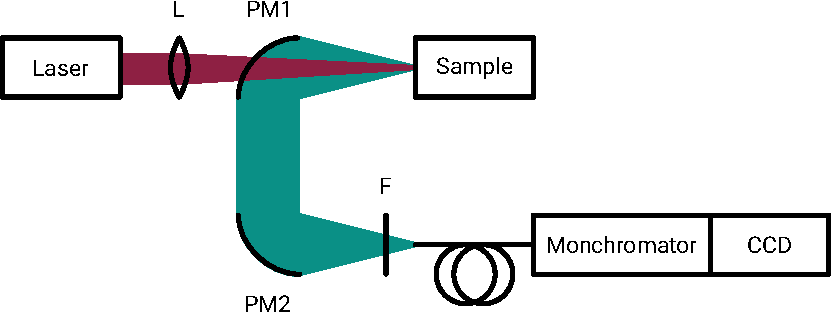
\includegraphics{figures/setup.pdf}
        \caption{Schematic}
    \end{subfigure}\hfill
    \begin{subfigure}{2in}
        \centering
        \includegraphics{figures/photo_setup.pdf}
        \caption{Photograph}
    \end{subfigure}
    \caption{Experimental setup used to measure thermal emission from ultrafast-excited hot electrons. The schematic shows the optical path and key components; the photograph shows the arrangement inside the chamber.}
    \label{fig:setup}
\end{figure}

The experimental setup, originally developed by Leon Roob~\cite{roob_thermal_2025}, is shown in \autoref{fig:setup}. It is designed to measure broadband thermal emission from hot electrons in graphite using reflective collection optics and a fibre-coupled spectrometer.

The excitation source is a PHAROS PH1-20 (Light Conversion) at a centre wavelength of \SI{1030}{\nano\metre}, with pulse duration \SI{250}{\femto\second} (FWHM) and repetition rate \SI{40}{\kilo\hertz}. The pulse energy is \SI{7.5}{\micro\joule} (average power \SI{300}{\milli\watt}). The beam pointing is stabilised in four axes and expanded to a diameter of \SI{5}{\milli\metre} before entering the chamber.

Inside the chamber, a plano-convex lens with focal length \(f=\SI{200}{\milli\metre}\) focuses the beam onto the sample. Using the standard diffraction estimate \(d \approx 4\lambda f / \pi D\) with \(\lambda=\SI{1030}{\nano\metre}\) and \(D=\SI{5}{\milli\metre}\), the expected spot diameter is \(\sim\SI{50}{\micro\metre}\).

The target is a graphite sample mounted on a three-axis translation stage. Thermal emission from the irradiated spot is collected by two off-axis parabolic mirrors (UV-enhanced aluminium). The first mirror (PM1, \(f=\SI{50}{\milli\metre}\)) collimates the emission; the second (PM2, \(f=\SI{101}{\milli\metre}\)) focuses it onto a band-pass filter and into a multimode fibre with a \SI{200}{\micro\metre} core (Ocean Optics QP200-2-SR-BX). The magnification is \(M = f_{\mathrm{PM2}}/f_{\mathrm{PM1}} \approx 2\), yielding an image spot of \(\sim\SI{100}{\micro\metre}\) at the fibre entrance, comfortably within the core.

The fibre feeds an Acton SpectraPro 300i monochromator equipped with a 150\,lines\,mm\(^{-1}\) grating blazed at \SI{500}{\nano\metre}. The dispersed spectrum is detected by an Andor iXon\textsuperscript{EM}+ 897 EMCCD operated in vertical binning mode, effectively serving as a 1D line detector.All spectra are corrected by subtracting a dark frame recorded with identical acquisition settings; this removes the fixed electronic bias (offset) and dark current.
Wavelength calibration (performed once following the manufacturer’s procedure~\cite{roob_thermal_2025}) was stable throughout the measurements.

For alignment and maximal throughput, the lens, sample, and fibre ferrule are mounted on independent precision translation stages, while PM1 and PM2 are fixed on the common optical axis. 

\section{Methods}

\subsection{Model}
\begin{table}
    \centering
    \begin{tabular}{lllll}
        Parameter & Symbol & Value & \\
        \hline
        Spot diameter on sample\footnote{State definition (FWHM or $1/\mathrm e^2$).} & $d_{\text{spot}}$ & $70^{+50}_{-0}$\;\si{\micro\metre}\\
        Pulse duration & $\tau_\text{fwhm}$ & \SI{250(50)}{fs} & \\
        Optical absorption depth & $d_{\text{abs}}$ & \SI{250(100)}{\nano\metre} &  &  \\
        Average laser power & $P_{\text{avg}}$ & \SI{300(5)}{mW} &  &  \\
        Repetition rate & $f_{\text{rep}}$ & \SI{40}{k\hertz} &  &  \\
        Cooling time constant & $\tau_{\mathrm{ep}}$ & \SI{250(50)}{fs} & \cite{stange_hot_2015} &  \\
        Electronic heat capacity & $C_e(T_e)$ & \si{\joule\per\metre\cubed\per\kelvin\squared} & \cite{nihira_temperature_2003} &  \\
        Lattice (ambient) temperature & $T_l$ & \SI{300}{\kelvin} & &  \\
    \end{tabular}
    \caption{Model parameters used in the spectrum calculation. Uncertainties in $1\sigma$.}
    \label{tab:parameters}
\end{table}

We obtain the electron temperature trajectory $T_e(t)$ by numerically integrating the ODE in the Theory section (\autoref{eq:Te}), using a Gaussian pulse for $P(t)$ with per-pulse energy $E_p = P_{\text{avg}}/f_{\text{rep}}$. The time step $\Delta t$ and integration window were chosen such that further refinement did not change the resulting spectrum appreciably. The parameters used are listed in \autoref{tab:parameters}.

The modeled spectral power density is then computed by inserting $T_e(t)$ into Planck’s law (Eq.~\eqref{eq:P}) and integrating numerically over time.

To estimate uncertainties, we sample the parameters in \autoref{tab:parameters} within their stated $1\sigma$ ranges, recompute the (relative) spectrum for each draw, and report, for each wavelength, the mean and standard deviation.


\subsection{Focusing and alignment}
The objective is to image the excited spot on the sample onto the spectrometer fibre with maximal, stable throughput. Parabolic mirrors (PM1/PM2) remain fixed once set; all focusing is done with the lamp, fibre/spectrometer port, and sample stages.

\begin{enumerate}
  \item \textbf{Remove the sample and place a fibre-coupled lamp at the sample position.}
  Mount the lamp so its ferrule sits at the exact $x$–$y$–$z$ location the sample surface will occupy. Use \emph{visible light} from the lamp to aid the initial alignment and viewing.

  \item \textbf{Align the lamp beam so the image at the spectrometer fibre port is circular and sharply focused.}
  With PM1/PM2 fixed on the common axis, adjust the lamp position and pointing until the spot at the fibre entrance appears round, centred, and with the smallest, sharp-edged footprint. This confirms the collection path is approximately aligned.

  \item \textbf{Connect the spectrometer to its port and maximise the signal.}
  Attach the collection fibre to the spectrometer entrance. Using live counts, \emph{slightly move the spectrometer (or fibre ferrule)} to find the coupling “sweet spot.” Then, use the \emph{micrometer screws on the sample/lamp stage} for fine $x$–$y$–$z$ adjustments to peak the signal. 
  \emph{Focused spot size:} at optimal focus the lamp image at the fibre face is circular and sharp, with a diameter on the order of \(\sim\)the expected image (\(\approx\)\SI{100}{\micro\metre} here, comfortably within the \SI{200}{\micro\metre} core). Record these stage coordinates.

  \item \textbf{Swap the lamp for the sample at the \emph{same} position.}
  Insert the sample so its surface coincides with the previously established plane (use a kinematic stop or gauge if available). Keep PM1/PM2 untouched.

  \item \textbf{Illuminate the sample via the lamp path and fine-focus the sample.}
  Temporarily reconnect the lamp to the spectrometer port so the sample is illuminated (reverse-path check). On the inspection optics, adjust the sample $z$ to \emph{minimise the visible spot size}; a sharply defined, smallest spot indicates correct focus in the PM1 object plane. Re-centre $x$–$y$ if needed.

  \item \textbf{Turn on the \SI{1030}{\nano\metre} laser and set the pump focus.}
  With the lamp off, use an IR viewing card to locate the pump on the sample. Adjust the focusing lens and sample $z$ to minimise the IR spot on the same surface plane. Start at low power to avoid damage; only increase after focus is established.

  \item \textbf{Disconnect the lamp and use the spectrometer to maximise the reflected-signal alignment.}
  With only the laser on, monitor the spectrometer signal (from scattered/reflected light) and perform small orthogonal scans: sample $z$ in tens of \si{\micro\metre}, and fibre $x$–$y$ within \(\pm\)\SI{50}{\micro\metre}. Fine-tune pump focus and sample/fibre positions for \emph{maximum} signal. Record final stage coordinates (sample $z$, fibre $x$–$y$) as the operational setpoint.
\end{enumerate}

\noindent\textit{Notes.}
Keep the spectrometer exposure and slit constant during focusing. Use the same wavelength setting throughout to avoid alignment bias. The “circular and sharply focused” lamp image at the fibre face is the quickest sanity check; if it degrades, re-do steps 1–3 before touching the mirrors.


\subsection{Noise and detector considerations}
Detecting the weak thermal radiation from hot electrons requires careful optimisation of the signal-to-noise ratio (SNR). In this setup the dominant noise sources originate from the detector; laser power fluctuations are treated as negligible. The EMCCD mechanisms are well documented by Andor~\cite{andor_establishing_nodate,dr_jo_walters_sensitivity_2023} and standardised terminology follows~\cite{european_machine_vision_association_standard_2010}.

\textbf{Readout noise.}
This is the fundamental floor from charge transfer and A/D conversion. For the present camera, the fit in \autoref{fig:dark_noise} yields a constant read noise of
\(\sigma_{\text{read}}=\SI{0.81(12)}{e^{-}}\), consistent with the manufacturer’s specification~\cite{andor_ixonem_nodate}.
Because read noise is applied \emph{per read} rather than per pixel, hardware \emph{vertical binning} (1D line-detector mode) reduces its impact by summing signal prior to the single read.

\textbf{Dark current noise.}
Thermally generated charge scales with temperature and time,
\(N_\text{dark}\propto \exp(-E/kT)\,t_\text{exp}\).
\autoref{fig:dark_noise} shows the measured dependence; fitting gives an effective activation energy \(E=\SI{0.597(4)}{eV}\).
With the sensor cooled to \SI{-80}{\degreeCelsius}, the dark contribution is negligible at the exposure times used.

\begin{figure}
    \centering
    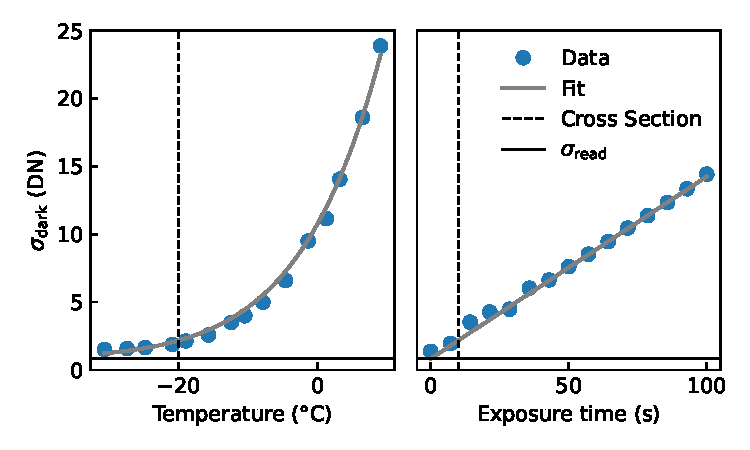
\includegraphics{../analysis/figures/dark_noise.pdf}
    \caption{Dark noise vs.\ sensor temperature and exposure time. Fit yields \(E=\SI{0.597(4)}{eV}\) and \(\sigma_{\text{read}}=\SI{0.81(12)}{e^{-}}\).}
    \label{fig:dark_noise}
\end{figure}

\textbf{Clock-induced charge (CIC).}
CIC is created during high-speed clocking.
Its apparent contribution grows with electron multiplication gain, so \emph{EM gain is disabled} in this work (signal levels are well above the read-noise floor), which keeps CIC negligible~\cite{andor_establishing_nodate}.

\textbf{Shot noise and photon-transfer method.}
Under these optimised conditions the dominant term is photon (shot) noise.
Incident photons create photoelectrons with quantum efficiency \(\eta\), so \(N_e=\eta\,N_{\text{photons}}\) and, for Poisson statistics, \(\operatorname{var}(N_e)=N_e\)~\cite{european_machine_vision_association_standard_2010}.
Let \(G\) denote the system conversion gain (DN per electron). The measured signal in data numbers (DN) is \(S = G\,N_e\), and the measured variance becomes \(\sigma^2_{\text{meas}} \;=\; \sigma_{\text{read}}^2 \;+\; G\,S\) (dark \& CIC negligible, no EM gain).
Thus a plot of variance vs.\ mean (photon-transfer curve) is linear in the shot-noise regime with slope \(G\).
\autoref{fig:shotnoise} shows this behaviour; from the slope we estimate \(G \approx 10~\text{DN}/e^{-}\).
Note that this procedure does \emph{not} determine \(\eta\); it only gives the DN-to-electron conversion.

\begin{figure}
    \centering
    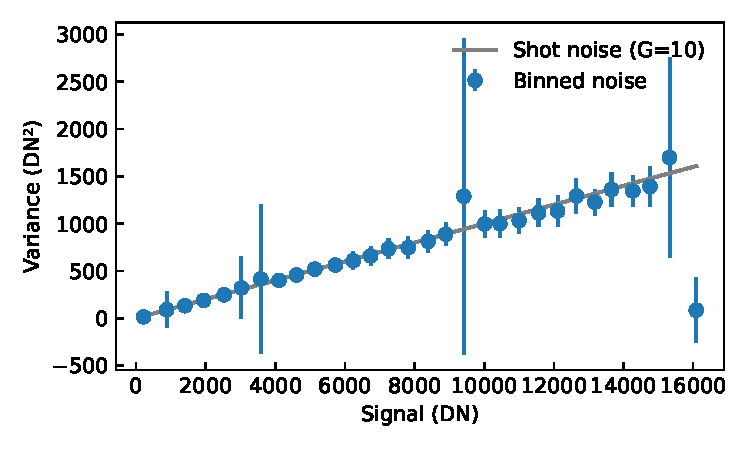
\includegraphics{../analysis/figures/shot noise.pdf}
    \caption{Measured noise vs.\ signal (photon-transfer curve) demonstrating shot-noise-limited operation; the linear slope yields the conversion gain \(G\).}
    \label{fig:shotnoise}
\end{figure}

\textbf{Practical settings for reproducibility.}
(1) Keep the camera at \(\leq\)\SI{-80}{\degreeCelsius}; (2) use vertical binning to treat the EMCCD as a 1D detector; (3) disable EM gain to avoid CIC and excess-noise-factor penalties; (4) fix slit width and exposure during noise characterisation; (5) verify the shot-noise regime by measuring \(\sigma^2\) vs.\ \(S\) and confirming linearity and slope \(G\)


\section{Results}
\begin{figure}
    \centering
    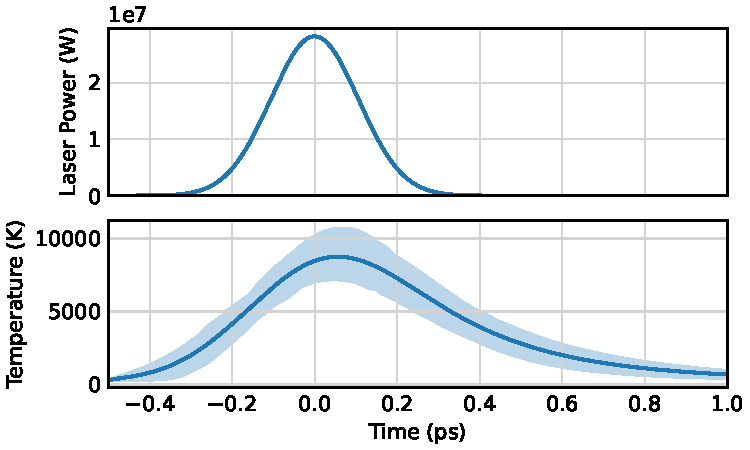
\includegraphics{../analysis/figures/model te.pdf}
    \caption{Gaussian pump \(S\) and computed electron temperature \(T_e(t)\) from the lumped two-temperature model (parameters in \autoref{tab:parameters}). The fast rise is followed by electron–phonon cooling with time constant \(\tau_{\mathrm{ep}}\). The shaded band shows the \(1\sigma\) Monte Carlo uncertainty.}
    \label{fig:Te}
\end{figure}
\begin{figure}
    \centering
    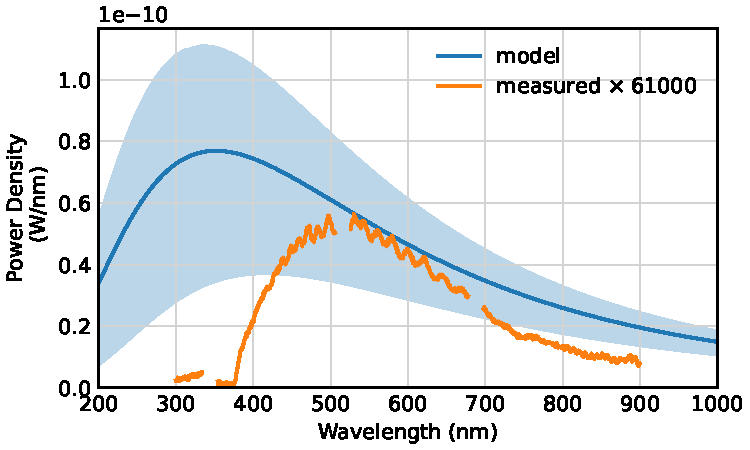
\includegraphics{../analysis/figures/spectrum de.pdf}
    \caption{Measured spectral power density \(P(\lambda)\) compared with the model spectrum obtained by applying Planck’s law to \(T_e(t)\). The measurement is scaled to match the model. The measured peak is narrower than the model, consistent with the instrument’s finite sensitivity window.}
    \label{fig:spectra}
\end{figure}
\begin{figure}
    \centering
    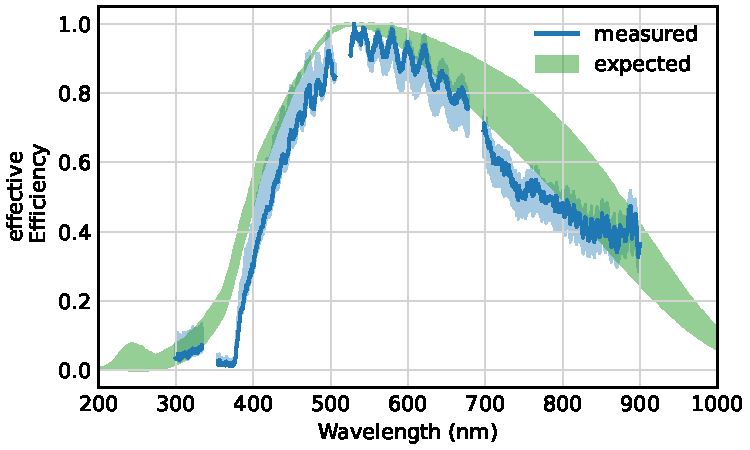
\includegraphics{../analysis/figures/efficiency de.pdf}
    \caption{Effective spectrometer efficiency (peak-normalised) from \(P^{\text{meas}}(\lambda)/P^{\text{model}}(\lambda)\). The overlay shows the expected relative efficiency from component specifications (camera QE \(\times\) blazed-grating model). The shaded range reflects uncertainty in blaze parameters. The measured curve shows stronger roll-off at both band edges and oscillations over wavelength.}
    \label{fig:efficiency}
\end{figure}

As shown in \autoref{fig:Te}, a Gaussian pump drives a rapid rise of the electron temperature \(T_e(t)\) according to \autoref{eq:Te}, followed by cooling on the electron–phonon timescale \(\tau_{\mathrm{ep}}\) using the parameters in \autoref{tab:parameters}. The shaded band (Monte Carlo) indicates the propagated uncertainty; the inferred peak temperature is \SI{8500(2500)}{\kelvin}.

Using \(T_e(t)\) as input to Planck’s law (\autoref{eq:P}), the modelled spectral power density \(P(\lambda)\) is computed and compared with the bias/dark-subtracted measurement in \autoref{fig:spectra}. Conversion from the measured signal to spectral power density follows
\begin{equation}
  P^{\text{meas}}(\lambda)
  = \frac{S(\lambda)}{G\,t_{\text{exp}}\,\Delta\lambda}\,\frac{hc}{\lambda},
\end{equation}
where \(S\) is in DN (bias/dark subtracted), \(G\) is the DN/\(e^-\) conversion gain, \(t_{\text{exp}}\) the exposure time, and \(\Delta\lambda\) the bin width. The factor \(hc/\lambda\) uses \(\lambda\) in \si{\metre} to yield units of \si{\watt\per\nano\metre}. The measured \(P(\lambda)\) is lower in absolute scale than the unscaled model; for visual comparison, the model in \autoref{fig:spectra} is multiplied by a constant to match the measured peak. The measured spectrum is noticeably narrower than the model, consistent with the finite sensitivity window set by the Si detector QE and the blazed-grating envelope.

An effective spectrometer efficiency is obtained by taking the wavelength-wise ratio \(P^{\text{meas}}(\lambda)/P^{\text{model}}(\lambda)\) and normalising to its maximum, so the peak equals unity (\autoref{fig:efficiency}). The expected curve is calculated from the manufacturer’s QE data for the camera when new~\cite{andor_ixonem_nodate} multiplied by a blazed-grating efficiency model~\cite{barker_ripple_1984}; the shaded interval reflects uncertainty in the blaze parameters. The measured efficiency falls off more steeply than expected at both short and long wavelengths, indicating additional wavelength-dependent loss not captured by the nominal QE\(\times\)blaze model. Moreover, the measured curve exhibits oscillations over wavelength, which may indicate interference effects or ripple in the grating efficiency.


\section{Discussion}
The earlier-than-expected roll-off at the short-wavelength edge of the effective efficiency curve (\autoref{fig:efficiency}) is plausibly explained by degradation of the UV-enhancing coating on the detector, consistent with the age of the EMCCD. At the long-wavelength edge, reduced response may arise from decreased detector quantum efficiency in the near-IR due to ageing-related changes in the Si surface passivation, as well as possible increased absorption in optical coatings. 

The oscillatory structure superimposed on the efficiency curve is consistent with thin-film interference effects, likely from oxide layers formed on metallic mirror surfaces and other coated optics. Such features are stable over time but can vary in amplitude and period depending on the exact thickness and refractive index of the oxidised layers.


\section{Discussion}
The earlier-than-expected roll-off at the short-wavelength edge of the effective efficiency (\autoref{fig:efficiency}) is plausibly due to degradation of the UV-enhancing coating on the detector, consistent with the instrument’s age. The long-wavelength roll-off may stem from reduced near-IR sensitivity of the EMCCD caused by ageing-related changes in the silicon surface passivation and anti-reflection coatings, compounded by increased absorption in optical coatings and possible fibre transmission losses.  

The oscillatory structure superimposed on the efficiency curve is consistent with thin-film interference effects, likely arising from oxide layers on metallic mirrors and other coated optics. Such features are stable over time but depend on the exact thickness and refractive index of the oxidised layers.

\section{Conclusion}
The present comparison between model and measurement is limited by the restricted sensitivity window of the existing optical path. A measurement with a calibrated, broadband setup is required to validate the model more rigorously. Furthermore, if the hot-electron emission mechanism is to be used for any serious calibration purpose, a more detailed physical model will be necessary to reduce uncertainty.  
Nevertheless, the principle of using hot electrons remains one of the most straightforward ways to generate broadband, predictable UV emission.


\clearpage
\printbibliography

\end{document}